% Synchronized to r45459
\section{The Packet Filter}
\configlabel{PF\_NEW\_CONFIG}{PFNEWCONFIG}

\newcommand{\fwaction}[1]{{\small\textsf{#1}}}
\newcommand{\fwchain}[1]{\texttt{#1}}
\newcommand{\fwtable}[1]{\textsc{#1}}
\newcommand{\fwmatch}[1]{\texttt{#1}}
\newcommand{\fwpktstate}[1]{\texttt{#1}}
\newcommand{\fwloglevel}[1]{\texttt{#1}}
\newcommand{\protocol}[1]{\texttt{#1}}
\newcommand{\host}[1]{\texttt{#1}}
\newcommand{\package}[1]{\texttt{#1}}

The Linux kernel used by fli4l provides a packet filter which controls
who is allowed to communicate with or through the Router. Furthermore,
things like port forwarding (a packet addressed to the router is
forwarded to another internal computer) and masquerading (packets
sent from a computer behind the router are changed to look as
if they came from the router itself) can be realized.

The structure of the packet filter is shown in Figure \ref{fig:netfilter}.\\

Packets arrive over a network interface and pass through the \fwchain{PREROUTING}-chain.
Here the packets addressed to the router are passed to another computer by
changing destination address and destination port. If the packet is
addressed to the router it is sent to the \fwchain{INPUT}-chain, if not, to the
\fwchain{FORWARD}-chain. Both chains will check if the packet is permitted.
If the packet is accepted, it is delivered to the local destination process
or passed via the \fwchain{POSTROUTING}-chain (in which packet masquerading is done)
to the network interface by which it can reach its target. Locally generated
packets are filtered in the \fwchain{OUTPUT}-chain and finally (if
successfully) also pass through the \fwchain{POSTROUTING}-chain to the
correct network interface.

\begin{figure}[htbp]
  \centering
  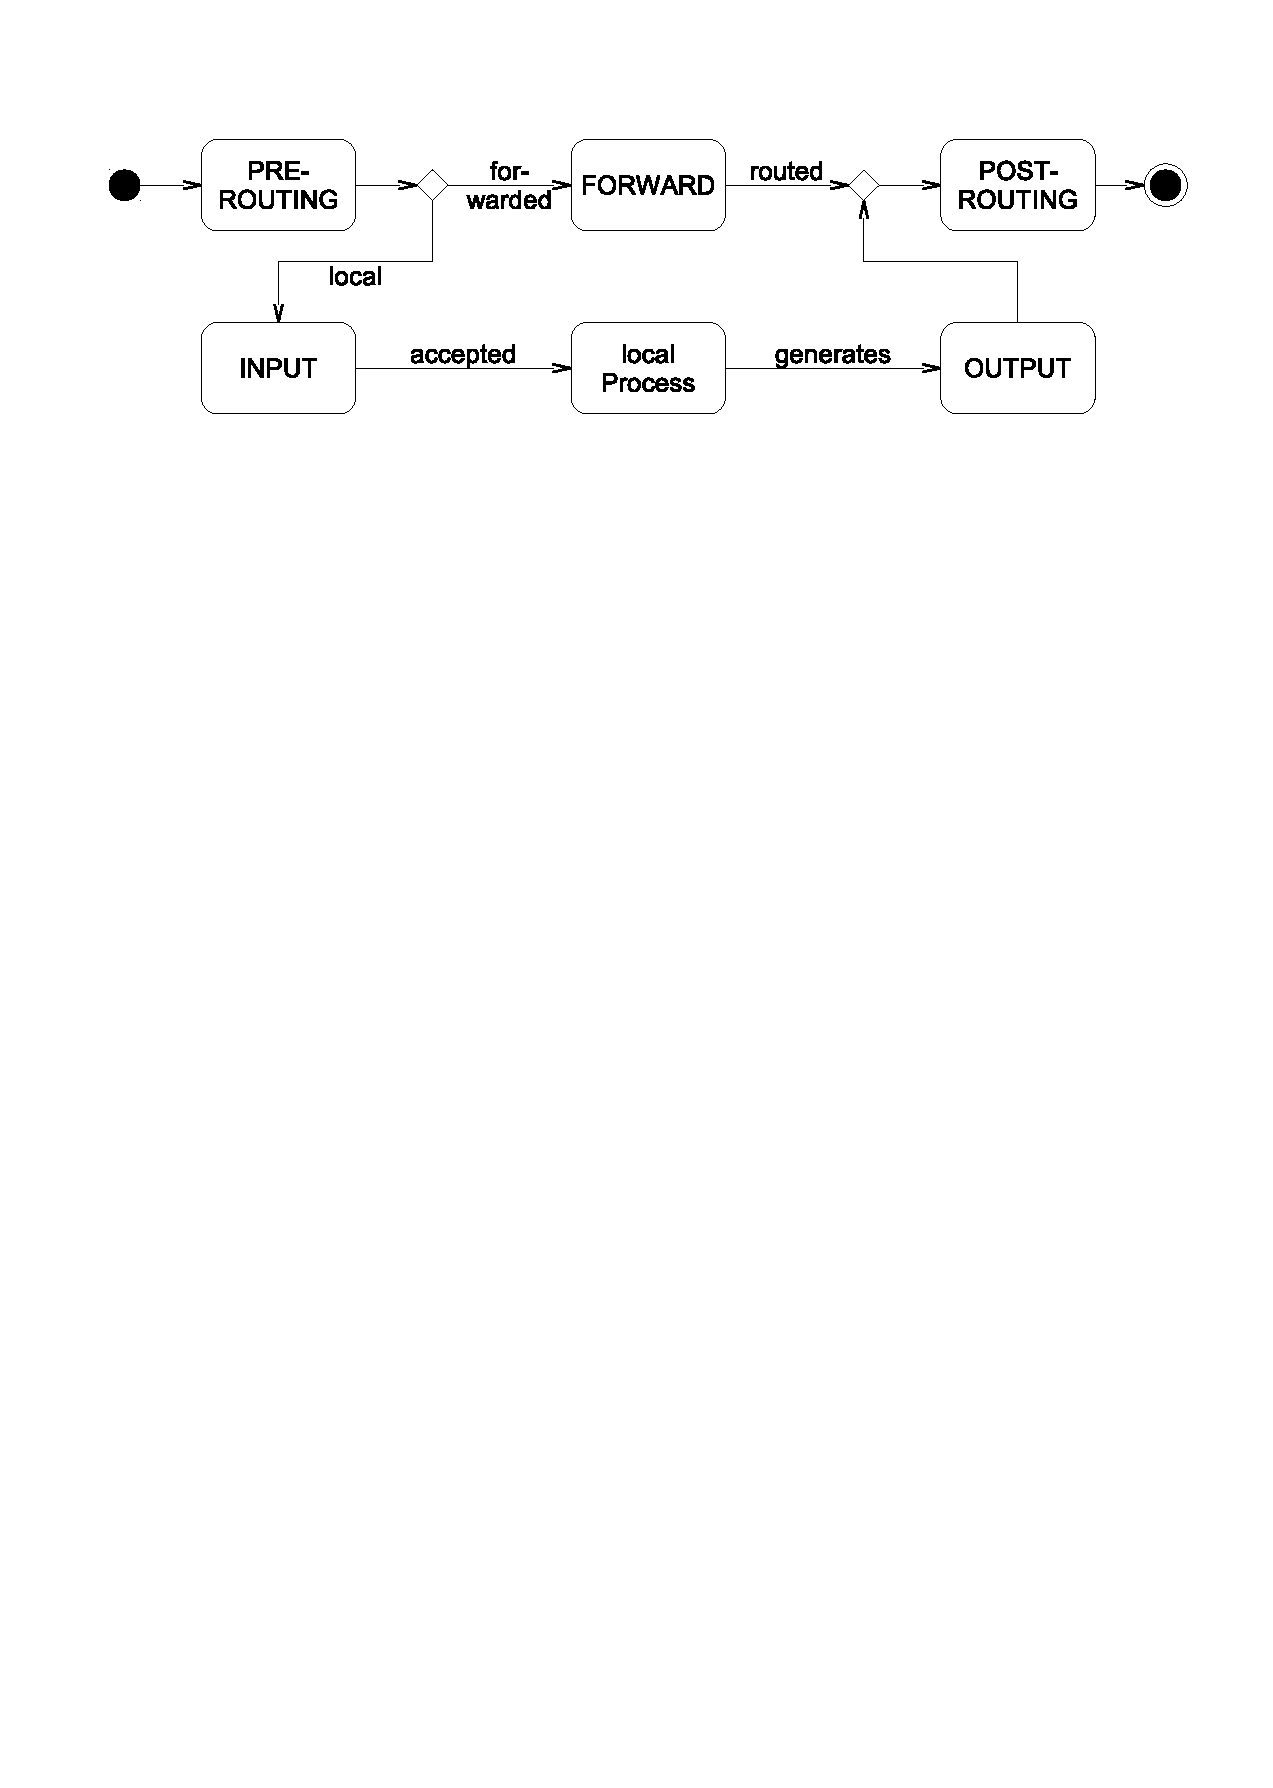
\includegraphics[width=\columnwidth]{firewall}
  \caption{Packet Filter Structure}
  \label{fig:netfilter}
\end{figure}

With the packet filter configuration, the individual chains of the 
packet filter can be modified directly. An individual array exists
for each chain, one for the
\fwchain{INPUT}-chain (\var{PF\_INPUT\_\%}), one for the
\fwchain{FORWARD}-chain (\var{PF\_FORWARD\_\%}), one for the
\fwchain{OUTPUT}-chain (\var{PF\_OUTPUT\_\%}), one for the
\fwchain{PREROUTING}-chain (managing port forwarding)
(\var{PF\_PREROUTING\_\%}), and one for the \fwchain{POSTROUTING}-chain,
managing packet masquerading (\var{PF\_POSTROUTING\_\%}).

An entry in one of these arrays consists mainly of an action (see below)
which can be restricted by additional conditions. These conditions
relate to properties of the considered packet. A packet contains
information about its origin (source PC that has sent the packet), 
its target (to which PC and which application should the packet be delivered)
and much more. Conditions can refer to the following properties of
a packet:

\begin{itemize}
  \item source (source address, source port or both)
  \item destination (destination address, destination port or both)
  \item protocol
  \item interface on which the packet comes in or goes out
  \item MAC-address of the originating PC
  \item state of the packet or the connection the packet comes from
\end{itemize}

If a packet comes in, the entries resp. the resulting rules generated
are processed from top to bottom and the first action to which all conditions
apply is performed. If none of the rules matches, the default action is executed,
which may be specified for (almost) any table.

An entry has the following format, bearing in mind that
all restrictions are optional:

\begin{example}
\begin{verbatim}
    restriction{0,} [[source] [destination]] action [BIDIRECTIONAL|LOG|NOLOG]
\end{verbatim}
\end{example}


At all points where networks, IP addresses or hosts need to be specified,
you can also refer to \var{IP\_NET\_\%}, \var{IP\_NET\_\%\_IPADDR} or
via \host{@hostname} to a host from \var{HOST\_\%}. If \var{OPT\_DNS}
is enabled, then outside of actions via \host{@fqdn} also hosts which
are \emph{nicht} mentioned in \var{HOST\_\%} can be referenced by their
names. This is particularly useful if dealing with external hosts which
also possess many (and changing) IP addresses.

\marklabel{sec:fwrules_actions}{\subsection{Packet Filter Actions}}

The following actions appy:
\begin{center}
    \begin{longtable}{|l|l|p{0.5\textwidth}|}
        \hline
        \multicolumn{1}{|l}{\textbf{Action}} &
        \multicolumn{1}{|l}{\textbf{chain(s)}} &
        \multicolumn{1}{|l|}{\textbf{Meaning}} \\
        \hline
        \endhead
        \hline
        \endfoot
        \endlastfoot
        \fwaction{ACCEPT}       & all
                                & Accept the packet.
                                \\
        \hline
        \fwaction{DROP}         &
                                \begin{tabular}[t]{@{}l@{}}
                                    \fwchain{INPUT} \\
                                    \fwchain{FORWARD} \\
                                    \fwchain{OUTPUT}
                                \end{tabular}
                                & Drop the packet (the sender recognizes that
                                just because no answer and no error message 
                                comes back).
                                \\
        \hline
        \fwaction{REJECT}       &
                                \begin{tabular}[t]{@{}l@{}}
                                    \fwchain{INPUT} \\
                                    \fwchain{FORWARD} \\
                                    \fwchain{OUTPUT}
                                \end{tabular}
                                & Reject the packet (the sender gets
                                a corresponding error message).
                                \\
        \hline
        \fwaction{LOG}          & all
                                & Log the packet and proceed to the next rule.
                                To distinguish log entries a prefix may be
                                used, specified by \fwaction{LOG:log-prefix}.
                                The maximum length of this prefix is 28
                                characters and it may contain letters, numbers,
                                hyphens (\texttt{-}), and underscores (\texttt{\_}).
                                \\
        \hline
        \fwaction{MASQUERADE}   & \fwchain{POSTROUTING}
                                & Mask the packet: Replace the source address
                                of the packet by the own one and make sure that
                                replies for this connection are redirected to 
                                the correct computer.
                                \\
        \hline
        \fwaction{SNAT}         & \fwchain{POSTROUTING}
                                & Replace source address and source port of the
                                packet by the address specified as a parameter
                                for \fwaction{SNAT} (for all packets belonging
                                to the connection in consideration).
                                \\
        \hline
        \fwaction{DNAT}         & \fwchain{PREROUTING}
                                & Replace destination address and destination port
                                of the packet by the address specified as a parameter
                                for \fwaction{SNAT} (for all packets belonging
                                to the connection in consideration).
                                \\
        \hline
        \fwaction{REDIRECT}     &
                                \begin{tabular}[t]{@{}l@{}}
                                    \fwchain{PREROUTING} \\
                                    \fwchain{OUTPUT}
                                \end{tabular}
                                & Replace destination port of the packet 
                                by the address specified as a parameter
                                for \fwaction{SNAT} (for all packets belonging
                                to the connection in consideration).
                                \\
        \hline
        \fwaction{NETMAP}       &
                                \begin{tabular}[t]{@{}l@{}}
                                    \fwchain{PREROUTING} \\
                                    \fwchain{POSTROUTING}
                                \end{tabular}
                                & Copy destination resp. source address of the
                                packet to the range specified as a parameter for
                                \fwaction{NETMAP}; the ports stay unchanged
                                (for all packets belonging to the connection 
                                in consideration; while changing the destination
                                address in the \fwchain{PREROUTING}-chain and the 
                                source address of the \fwchain{POSTROUTING}-chain).
                                \\
        \hline
        \caption{Packet Filter Actions}\marklabel{fwrule:actions}{}
    \end{longtable}
\end{center}

Some of these actions may be modified in behaviour by using the options 
\fwaction{BIDIRECTIONAL}, \fwaction{LOG} or \fwaction{NOLOG}.
\fwaction{BIDIRECTIONAL} generates the same rule a second time with
source and destination adresse exchanged (and source and destination
port exchanged and/or in- and outbound network interface exchanged if
specified). \fwaction{LOG}/\fwaction{NOLOG} activates resp. deactivates
logging for this rule.

\marklabel{sec:fwrules_limits}{\subsection{Restrictions For Rules}}

Restrictions may be defined by constraints explained in the following sections.
You may use \fwmatch{any} at any place where you don't want restrictions but
want/have to specify something. Constraints can be specified in any order
if they have a preceding prefix. This applies to all restrictions, except
for specifying a source or destination address which must always be placed
directly in front of the action, other constraints must be specified before.
Restrictions can also be negated, simply prefix them by a \fwmatch{!}.

\subsubsection{Constraints For Source And Target}

Each packet contains source and target informations in a tuple of an IP address and
ports.\footnote{A port only exists for TCP- and UDP-packets.} This source resp.
target can serve as a constraint and may be addressed like this:

\begin{center}
    \begin{longtable}{|l|p{0.5\textwidth}|}
        \hline
        \multicolumn{1}{|l}{\textbf{Expression}} &
        \multicolumn{1}{|l|}{\textbf{Meaning}} \\
        \hline
        \endhead
        \hline
        \endfoot
        \endlastfoot
    \verb+ip+               & a simple IP address\\
    \verb+network+          & a network declaration in the form of \verb+<ip>/<netmask>+ \\
    \verb+port[-port]+      & a port resp. a port range\\
    \verb+IP_NET_x_IPADDR+  & the IP address of the \verb+x+ router's interface\\
    \verb+IP_NET_x+         & the \verb+x+ router's subnet\\
    \verb+IP_ROUTE_x+       & the subnet \verb+x+ specified in the route
      (default routes can't be used, they would match \fwmatch{any} and are excluded precautiously)\\
    \verb+@name+            & one of the names or aliases set via HOST\_\%\_*; 
			      the associated IP address will be filled in here\\
    \verb+<ip oder netzwerk>:port[-port]+ & Host- resp. network address in one of the variants
			    above, combined with a port resp. port range\\
        \hline
        \caption{Constraints For Source And Target In Paket Filter Rules}
    \end{longtable}
\end{center}

\noindent Example: \verb+'192.168.6.2 any DROP'+

If two of these lines shine up the first will be considered as source
and the second as target. Hence, in this example we drop the packets
originating from the computer with the IP address 192.168.6.2, regardless
of where they are targeted.

If only one line exists the decision if target or source is meant will
be made depending on the value, which is quite easy:
\begin{itemize}
  \item If it contains a port value, target is meant,
  \item in all other cases the source is.
\end{itemize}

If you would like to shorten the example above you could write
\verb+'192.168.6.2 DROP'+. No port is mentioned, hence the constraint
is valid for the source (the machine the packet originated from).

If we were to allow communication with the \protocol{ssh}-deamon, we could
write \verb+'any any:22 ACCEPT'+ (packets from any machine to \protocol{ssh}-port
22 of any machine will be accepted) or even shorter \verb+'22 ACCEPT'+. Only
a port is mentioned, hence we address the target and thus all packets
targeted to port 22.

For simplification you may append \fwaction{BIDIRECTIONAL} to the action to
express that the rule is valid for both communication directions. Then rules
will be generated with source and target addresses and if applicable ports
and network interfaces exchanged while leaving the rest untouched.

Examples:
\medskip

\begin{example}
\noindent
{\footnotesize
 \begin{tabular}{@{}p{5cm}p{10cm}@{}}
    \verb+127.0.0.1 ACCEPT+             & local communication (source 127.0.0.1) is allowed\\
    \verb+any 192.168.12.1 DROP+        & packets to address 192.168.12.1 will be dropped\\
    \verb+any 192.168.12.1 DROP LOG+    & packets to address 192.168.12.1 will be dropped and logged additionally\\
    \verb+any 192.168.12.1 DROP NOLOG+  & packets to address 192.168.12.1 will be dropped but not logged\\
    \verb+22 ACCEPT+                    & packets to port 22 (\protocol{ssh}) will be accepted\\
    \verb+IP_NET_1_NET ACCEPT+          & packets from the subnet connected to the first interface will be accepted\\
    \verb+IP_NET_1_NET IP_NET_2_NET+    & communication between the subnets connected to the first and second\\
    \verb+  ACCEPT BIDIRECTIONAL+       & interface are allowed\\
 \end{tabular}
}
\end{example}

\subsubsection{Interface Constraints}

A rule can be restricted concerning the Interface on which a packet
was received resp. will be transmitted. The format is as follows:
\fwmatch{if:}\emph{in}\fwmatch{:}\emph{out}

In the \fwchain{INPUT}-chain the interface for outbound packets is not
restrictable (the packet does not leave anyway), in the \fwchain{POSTROUTING}-chain
the interface for received packets is not restrictable, because the
informations about it do not exist anymore. Only in the \fwchain{FORWARD}-chain
constraints for both can be defined.

Possible values for \emph{in} resp. \emph{out}:

\begin{itemize}
  \item \fwmatch{lo} (Loopback-interface, local communication on the router)
  \item \verb+IP_NET_x_DEV+
  \item \fwmatch{pppoe} (the PPPoE-interface; only with package \package{dsl}
		or \package{pppoe\_server} activated).
  \item \fwmatch{any}
\end{itemize}

\subsubsection{Protocol Constraints}

A rule can be restricted concerning the protocol a packet belongs to.
The format is as follows:
\fwmatch{prot:}\emph{protocol} resp. \fwmatch{prot:}\emph{icmp}\fwmatch{:}\emph{icmp-type}.
\emph{protocol} can be set to one of the following values:

\begin{itemize}
  \item \fwmatch{tcp}
  \item \fwmatch{udp}
  \item \fwmatch{gre} (Generic Routing Encapsulation)
  \item \fwmatch{icmp} (additionally you can specify a name for the ICMP-type to be filterd (\fwmatch{echo-reply} or
    \fwmatch{echo-request}), i.e. \fwmatch{prot:icmp:echo-request})
  \item numeric value of the protocol-ID (i.e. 41 for IPv6)
  \item \fwmatch{any}
\end{itemize}

If such a constraint does not exists, but port numbers should
be used in a rule, then the rule is generated \emph{twice},
once for the \protocol{tcp} and once for the \protocol{udp} protocol.

\subsubsection{MAC-Address Constraints}

Via \fwmatch{mac:}\emph{mac-address} constraints based on the MAC  address
may be specified.

\subsubsection{Packet State Constraints}

fli4l's packet filter gathers informations on the state of connections.
This informations can be used to filter packets, i.e let only packets pass that
belong to connections already existing. The state of a connection can take
this values:\footnote{see \altlink{http://www.sns.ias.edu/~jns/files/iptables_talk/x38.htm}
for a detailed description}

\begin{center}
    \begin{longtable}{|l|p{0.7\textwidth}|}
        \hline
        \multicolumn{1}{|l}{\textbf{State}} &
        \multicolumn{1}{|l|}{\textbf{Meaning}} \\
        \hline
        \endhead
        \hline
        \endfoot
        \endlastfoot
        \fwpktstate{INVALID}        & The packet does not belong to a know connection.
                                    \\
        \fwpktstate{ESTABLISHED}    & The packet belongs to a connection, where
                                    packets have already been transmitted in both
                                    directions.
                                    \\
        \fwpktstate{NEW}            & The packet has established a new connection
                                    or belongs to a connection that did not have
                                    packets transmitted in both directions.
                                    \\
        \fwpktstate{RELATED}        & The packet establishes a new connection,
                                    but has a relation to an already existing
                                    connection (i.e. \protocol{ftp} establishes
                                    a separate connection for data transfer).
                                    \\
        \hline
        \caption{Packet State Constraints in Packet Filter Rules}
    \end{longtable}
\end{center}

States are defined as follows:
\fwmatch{state:}\emph{state(s)}. If you want to specify more than one
state they have to be separated by commas. I.e. to let packets
pass that belong directly or indirectly to established connections
write \fwmatch{state:}\fwpktstate{ESTABLISHED,RELATED} (this makes
sense in \fwchain{INPUT}- or \fwchain{FORWARD}-chain).

\subsubsection{Constraints Based On The Frequency Of Actions}

Under certain circumstances you may wish to restrict the frequency of
actions, i.e. allow only one ICMP-Echo request per second. This may be
reached with \fwmatch{limit}-constraints, which look like this:
\fwmatch{limit:}\emph{Frequency:Burst}. The frequency is specified as
\emph{n/time units} (second, minute, hour, day), however, events may also occur
in rapid succession (Burst). \texttt{limit:3/minute:5} for example means
that a maximum of three events per minute is allowed, but also five events
in rapid succession will be accepted.

\marklabel{sec:templates}{\subsection{Using Templates With The Packet Filter}}

To simplify dealing with the packet filter you may summarize rules frequently
occuring in templates. Thus, it is possible to provide a wide range of
packet filtering rules and combine them in a collection with a symbolic
name. Instead of directly using protocols and port numbers, you may then
use entries such as \fwmatch{tmpl:ssh} if you want to use the \protocol{ssh}
protocol in a rule. How to deal with templates is shown here using the
example of \protocol{ssh}.

If you want to reach your fli4l from the Internet via \protocol{ssh},
write into an entry in the array variable \var{PF\_input\_\%} the
corresponding service name (here \protocol{ssh}) preceded by
\fwmatch{tmpl} and the action to apply for this service. Example:

\begin{example}
\begin{verbatim}
    PF_INPUT_2='tmpl:ssh ACCEPT'
\end{verbatim}
\end{example}

\fwmatch{tmpl:} means that the rule should be based on a template. Specify the
name of the service after the `:', adapted to our example hence \protocol{ssh}.
At last you have to set an action to be bound to the service. Since we want to
acces the fli4l over the internet, we allow the connection with \fwaction{ACCEPT}.
Restrictions for IP-addresses or nets are not provided so the \protocol{ssh}-service
will be accessible on all interfaces from all networks. If you want to invoke further
restrictions for accessing the \protocol{ssh}-service you may use the packet filter
notation already explained above.

For which services rules are predefined (e.g. templates exist) can be seen
in the template file at \verb+opt/etc/fwrules.tmpl/templates+. A list in a table
follows (see table \ref{tab:fwrules_tmpl}).

\begin{center}
  {\footnotesize
  \begin{longtable}{|lll|}
     \hline
     {\textbf{Template}} & {\textbf{Protocol}} & {\textbf{Port(s)}} \\
     \hline\hline
     \endhead
     \input{fwrules_tmpl_table.inc} \\
     \hline
     \caption{Templates Included With fli4l}
     \label{tab:fwrules_tmpl}
  \end{longtable}}
\end{center}

The Syntax for this kind of packet filter rules is

\begin{example}
\begin{verbatim}
    tmpl:<Name of the service> <Constraint> <Action>
\end{verbatim}
\end{example}

\verb+<Constraint>+ allows everything mentioned at \ref{sec:fwrules_limits}.
Possible values for \verb+<Action>+ are listed and described 
in \ref{sec:fwrules_actions}.

Some more examples should clarify the process. At first let's have a look at \var{PF\_PREROUTING}:

\begin{example}
\begin{verbatim}
    PF_PREROUTING_N='2'
    PF_PREROUTING_1='tmpl:xbl dynamic DNAT:@xbox'
    PF_PREROUTING_2='tmpl:https dynamic DNAT:192.168.193.250'
\end{verbatim}
\end{example}

The rule \var{PF\_PREROUTING\_1} supplies the Xbox with everything necessary
for Xbox Live. By the use of \fwmatch{tmpl:xbl} all ports and protocols used
for Xbox Live will be forwarded to the \host{xbox}. Instead of using an IP
address we use an entry from the \var{HOST\_\%\_NAME}-array. \fwmatch{dynamic}
tells the fli4l to forward all ports from the internet interface.

The second rule forwards the \protocol{https}-protocol to a webserver in a DMZ
(Demilitarized Zone).

No let's have a look at \var{PF\_INPUT}:

\begin{example}
\begin{verbatim}
    PF_INPUT_N='3'
    PF_INPUT_1='if:IP_NET_1_DEV:any ACCEPT'
    PF_INPUT_2='if:pppoe:any prot:tcp 113 ACCEPT'
    PF_INPUT_3='if:br0:any tmpl:dns @xbox IP_NET_1_IPADDR ACCEPT'
\end{verbatim}
\end{example}

The first rule allows access to the router for everyone from the net defined 
in \var{IP\_NET\_1}. The second rule opens the \protocol{ident}-port needed
for package \package{oident}. The third rule allows the xbox to access fli4l's
DNS server. Notice the use of a host alias here.

\var{PF\_FORWARD} and \var{PF\_POSTROUTING} do not provide
\fwmatch{tmpl}-specific content.

\begin{figure}[htbp]
  \centering
  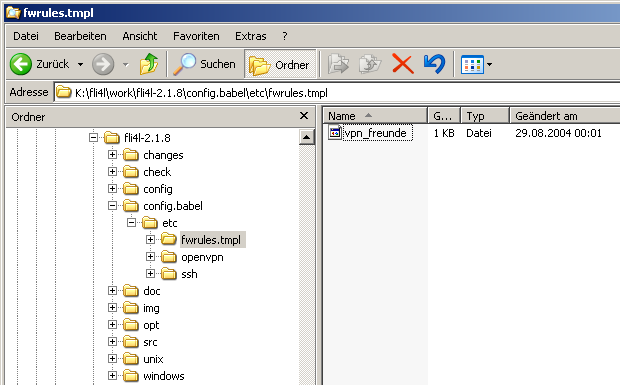
\includegraphics[width=0.9\columnwidth]{etc_fwrules_tmpl_dir}
  \caption{Directory Structure fli4l}
  \label{fig:etc_fwrules_tmpl_dir}
\end{figure}

It is also possible to create templates yourself or for other packages to
provide their own ones. To create a template you only need to create a text
file with the rules in it and name it like the template. For a private template
file use the directory \verb+etc/fwrules.tmpl+ (create it if necessary) under
your \texttt{config} directory as shown in picture \ref{fig:etc_fwrules_tmpl_dir}. 
Package developers or users needing templates for more than one configuration
may place their template files directly in \texttt{opt/etc/fwrules.tmpl}. 
The templates in the user's \texttt{config} directory override other settings, though.
The templates included in fli4l will be interpreted as the last ones. This enables you to
\glqq{}override\grqq{} fli4l's templates when providing templates by
the same name in your \texttt{config}-directory.

If, for example you like to create the template \fwmatch{vpn\_friends}, create a
file by the name \texttt{vpn\_friends}. The template should contain the services
\protocol{ssh}, \protocol{smtp}, \protocol{dns} and \protocol{samba}.
Hence you write the following to \texttt{vpn\_friends}:

\begin{example}
\begin{verbatim}
    prot:tcp 22
    prot:tcp 25
    53
    prot:udp 137-138
    prot:tcp 139
    prot:tcp 445
\end{verbatim}
\end{example}

\noindent Every time you use the template \fwmatch{vpn\_friends} rules will be
created for all contained protocols and ports.
\verb+PF_FORWARD_x='tmpl:vpn_friends ACCEPT'+ will create theses
\fwchain{FORWARD}-rules:

\begin{example}
\begin{verbatim}
    prot:tcp 22 ACCEPT
    prot:tcp 25 ACCEPT
    53 ACCEPT
    prot:udp 137-138 ACCEPT
    prot:tcp 139 ACCEPT
    prot:tcp 445 ACCEPT
\end{verbatim}
\end{example}

\subsection{Configuration Of The Packet Filter}

The packet filter is mainly configured by four array-variables:

\begin{itemize}
  \item \var{PF\_INPUT\_\%} configures the \fwchain{INPUT}-chain,
  \item \var{PF\_FORWARD\_\%} configures the \fwchain{FORWARD}-chain,
  \item \var{PF\_OUTPUT\_\%} configures the \fwchain{OUTPUT}-chain,
  \item \var{PF\_PREROUTING\_\%} configures the \fwchain{PREROUTING}-chain and
  \item \var{PF\_POSTROUTING\_\%} configures the \fwchain{POSTROUTING}-chain.
\end{itemize}

\configlabel{PF\_LOG\_LEVEL}{PFLOGLEVEL} For all chains following applies
the setting of the protocol level in \var{PF\_LOG\_LEVEL}, which may be
set to one of these values: \fwloglevel{debug}, \fwloglevel{info}, \fwloglevel{notice},
\fwloglevel{warning}, \fwloglevel{err}, \fwloglevel{crit}, \fwloglevel{alert},
\fwloglevel{emerg}.

\subsubsection{Then \fwchain{INPUT}-Chain}

The \fwchain{INPUT}-chain defines who is allowed to access the router.
If no rule of the \fwchain{INPUT}-chain matches, the default action
handles the packet and the protocol variable decides wheter a rejection
will be written to the system-protocol or not.

The following restrictions apply to the parameters:
\begin{itemize}
  \item Only \fwaction{ACCEPT}, \fwaction{DROP} and \fwaction{REJECT}
    can be specified as actions.
  \item If using interface constraints only the receiving
    interface can be restricted.
\end{itemize}

\begin{description}
\config{PF\_INPUT\_POLICY}{PF\_INPUT\_POLICY}{PFINPUTPOLICY}
This variable describes the default action to be taken if no other
rule applies. Possible values:

\begin{itemize}
\item \fwaction{ACCEPT} (not recommended)
\item \fwaction{REJECT}
\item \fwaction{DROP} (not recommended)
\end{itemize}

\config{PF\_INPUT\_ACCEPT\_DEF}{PF\_INPUT\_ACCEPT\_DEF}{PFINPUTACCEPTDEF}
If this variable is set to `yes' default rules will be generated needed for
the correct function of the router. Use `yes' as a default here.

If you want to configure the router's behaviour completely yourself you may
enter `no' here but you will have to define all rules on your own then.
An equivalent to the default behaviour would look like this (the explanation
of user defined chains can be found \jump{sec:userlists}{here}):

\begin{example}
{\footnotesize
\begin{verbatim}
    PF_INPUT_ACCEPT_DEF='no'
    #
    # limit ICMP echo requests - use a separate chain
    #
    PF_USR_CHAIN_N='1'
    PF_USR_CHAIN_1_NAME='usr-in-icmp'
    PF_USR_CHAIN_1_RULE_N='2'
    PF_USR_CHAIN_1_RULE_1='prot:icmp:echo-request length:0-150 limit:1/second:5 ACCEPT'
    PF_USR_CHAIN_1_RULE_2='state:RELATED ACCEPT'

    PF_INPUT_N='4'
    PF_INPUT_1='prot:icmp usr-in-icmp'
    PF_INPUT_2='state:ESTABLISHED,RELATED ACCEPT'
    PF_INPUT_3='if:lo:any ACCEPT'
    PF_INPUT_4='state:NEW 127.0.0.1 DROP BIDIRECTIONAL'
\end{verbatim}}
\end{example}

The first rule branches to the rate limited ``usr-in-icmp''-chain.
The second only accepts packets belonging to established connections
(packets that have either the state \fwpktstate{ESTABLISHED} or
\fwpktstate{RELATED}), and the third one allows local communication
(\verb+if:lo:any ACCEPT+). The fourth filters packets that pretend to
be local communication but are not accepted by the rules defined before.

If you work with OpenVPN, the rules have to be enhanced to enable packets used
by the chains there.

\begin{example}
\begin{verbatim}
    PF_INPUT_N='5'
    ...
    PF_INPUT_5='ovpn-chain'
\end{verbatim}
\end{example}

\config{PF\_INPUT\_LOG}{PF\_INPUT\_LOG}{PFINPUTLOG}
Defines if rejected packets should be logged by the kernel.
Log output can be directed to the syslog deamon by activating \var{OPT\_KLOGD}.

\config{PF\_INPUT\_LOG\_LIMIT}{PF\_INPUT\_LOG\_LIMIT}{PFINPUTLOGLIMIT}
Defines how often log entries will be generated. The frequency is described
as \emph{n/time units} with bursts in analog to the limit constraints, e.g.
\texttt{3/minute:5}. If this entry is empty a default of \texttt{1/second:5}
is used, if set to \texttt{none}, the limit constraints are disabled.

\configlabel{PF\_INPUT\_UDP\_REJ\_LIMIT}{PFINPUTUDPREJLIMIT}
\config{PF\_INPUT\_REJ\_LIMIT PF\_INPUT\_UDP\_REJ\_LIMIT}{PF\_INPUT\_REJ\_LIMIT}{PFINPUTREJLIMIT}
Specifies how often a \fwaction{REJECT}-packet is generated when rejecting
incoming packets. The frequency is described as \emph{n/time units} with bursts 
in analog to the limit constraints, e.g. \texttt{3/minute:5}. If this entry is
empty a default of \texttt{1/second:5} is used, if set to \texttt{none},
the limit constraints are disabled.

\config{PF\_INPUT\_ICMP\_ECHO\_REQ\_LIMIT}{PF\_INPUT\_ICMP\_ECHO\_REQ\_LIMIT}{PFINPUTICMPECHOREQLIMIT}
Defines how often fli4l should react to a ICMP-Echo-request.The frequency is
described as \emph{n/time units} with bursts in analog to the limit constraints,
e.g. \texttt{3/minute:5}. If the limit is reached packets will be ignored
(\fwaction{DROP}). If this entry is empty a default of \texttt{1/second:5}
is used, if set to \texttt{none}, the limit constraints are disabled.

\config{PF\_INPUT\_ICMP\_ECHO\_REQ\_SIZE}{PF\_INPUT\_ICMP\_ECHO\_REQ\_SIZE}{PFINPUTICMPECHOREQSIZE}
Defines the allowed size of an ICMP-Echo-request (in bytes). The packet header
has to be included in this setting besides the pure data. The default is 150 bytes.

\configlabel{PF\_INPUT\_x}{PFINPUTx}
\configlabel{PF\_INPUT\_x\_COMMENT}{PFINPUTxCOMMENT}
\config{PF\_INPUT\_N PF\_INPUT\_x PF\_INPUT\_x\_COMMENT}{PF\_INPUT\_N}{PFINPUTN}
A list of rules that describe which packets the router should accept resp. reject.
\end{description}

\subsubsection{The \fwchain{FORWARD}-Chain}

By using the \fwchain{FORWARD}-chain will be configured which packets are
forwarded by the router. If no rule of the \fwchain{FORWARD}-chain matches,
the default action handles the packet and the protocol variable decides
wheter a rejection will be written to the system-protocol or not.

With the used parameters the restriction applies that only the actions
\fwaction{ACCEPT}, \fwaction{DROP} and \fwaction{REJECT} are allowed.

\begin{description}
\config{PF\_FORWARD\_POLICY}{PF\_FORWARD\_POLICY}{PFFORWARDPOLICY}
This variable describes the default action to be taken if no other
rule applies. Possible values:

\begin{itemize}
\item \fwaction{ACCEPT}
\item \fwaction{REJECT}
\item \fwaction{DROP}
\end{itemize}

\config{PF\_FORWARD\_ACCEPT\_DEF}{PF\_FORWARD\_ACCEPT\_DEF}{PFFORWARDACCEPTDEF}
Determines if the router accepts packets belonging to established
connections. If this variable is set to `yes', fli4l generates
a rule for accepting packets of the according state automatically:

\verb+'state:ESTABLISHED,RELATED ACCEPT'+,

aswell as a rule to drop packets of unknown state:

\verb+'state:INVALID DROP'+.

and at last a rule to drop packets with faked IP addresses:

\verb+'state:NEW 127.0.0.1 DROP BIDIRECTIONAL'+.

In addition the other subsystems will generate some default rules~-- a
configuration without default rules with port forwarding and OpenVPN 
would contain at least the following rules:

\begin{example}
\begin{verbatim}
    PF_FORWARD_ACCEPT_DEF='no'
    PF_FORWARD_N='5'
    PF_FORWARD_1='state:ESTABLISHED,RELATED ACCEPT'
    PF_FORWARD_2='state:INVALID DROP'
    PF_FORWARD_3='state:NEW 127.0.0.1 DROP BIDIRECTIONAL'
    PF_FORWARD_4='pfwaccess-chain'
    PF_FORWARD_5='ovpn-chain'
\end{verbatim}
\end{example}

\config{PF\_FORWARD\_LOG}{PF\_FORWARD\_LOG}{PFFORWARDLOG}
Defines if rejected packets should be logged by the kernel.
Log output can be directed to the syslog deamon by activating \var{OPT\_KLOGD}.

\config{PF\_FORWARD\_LOG\_LIMIT}{PF\_FORWARD\_LOG\_LIMIT}{PFFORWARDLOGLIMIT}
Defines how often log entries will be generated. The frequency is described
as \emph{n/time units} with bursts in analog to the limit constraints, e.g.
\texttt{3/minute:5}. If this entry is empty a default of \texttt{1/second:5}
is used, if set to \texttt{none}, the limit constraints are disabled.

\configlabel{PF\_FORWARD\_UDP\_REJ\_LIMIT}{PFFORWARDUDPREJLIMIT}
\config{PF\_FORWARD\_REJ\_LIMIT PF\_FORWARD\_UDP\_REJ\_LIMIT}{PF\_FORWARD\_REJ\_LIMIT}{PFFORWARDREJLIMIT}
Specifies how often a \fwaction{REJECT}-packet is generated when rejecting
incoming packets. The frequency is described as \emph{n/time units} with bursts 
in analog to the limit constraints, e.g. \texttt{3/minute:5}. If this entry is
empty a default of \texttt{1/second:5} is used, if set to \texttt{none},
the limit constraints are disabled.

\configlabel{PF\_FORWARD\_x}{PFFORWARDx}
\configlabel{PF\_FORWARD\_x\_COMMENT}{PFFORWARDxCOMMENT}
\config{PF\_FORWARD\_N PF\_FORWARD\_x PF\_FORWARD\_x\_COMMENT}{PF\_FORWARD\_N}{PFFORWARDN}
A list of rules that describe which packets the router should forward resp. reject.

\end{description}

\subsubsection{The \fwchain{OUTPUT}-Chain}

The \fwchain{OUTPUT}-chain configures what the router is allowed to access. 
If no rule of the \fwchain{OUTPUT}-chain matches,
the default action handles the packet and the protocol variable decides
wheter a rejection will be written to the system-protocol or not.

With the used parameters the following restrictions apply:
\begin{itemize}
  \item Only \fwaction{ACCEPT}, \fwaction{DROP} and \fwaction{REJECT}
    can be specified as actions.
  \item For interface constraints only the output interface can
    be restricted.
\end{itemize}

\begin{description}
\config{PF\_OUTPUT\_POLICY}{PF\_OUTPUT\_POLICY}{PFOUTPUTPOLICY}
This variable describes the default action to be taken if no other
rule applies. Possible values:

\begin{itemize}
\item \fwaction{ACCEPT}
\item \fwaction{REJECT}
\item \fwaction{DROP}
\end{itemize}

\config{PF\_OUTPUT\_ACCEPT\_DEF}{PF\_OUTPUT\_ACCEPT\_DEF}{PFOUTPUTACCEPTDEF}
If this variable is set to `yes' default rules necessary for correct function of
the router will be generated. Use `yes' as a default here.

If you want to configure the router's behaviour completely yourself you may
enter `no' here but you will have to define all rules on your own then.
An equivalent to the default behaviour would look like this:

\begin{example}
{\footnotesize
\begin{verbatim}
    PF_OUTPUT_ACCEPT_DEF='no'

    PF_OUTPUT_N='1'
    PF_OUTPUT_1='state:ESTABLISHED,RELATED ACCEPT'
\end{verbatim}}
\end{example}

This single rule accepts only packets belonging to established connections
(e.g. packets of the state \fwpktstate{ESTABLISHED} or \fwpktstate{RELATED}).

\config{PF\_OUTPUT\_LOG}{PF\_OUTPUT\_LOG}{PFOUTPUTLOG}
Defines if rejected packets should be logged by the kernel.
Log output can be directed to the syslog deamon by activating \var{OPT\_KLOGD}.

\config{PF\_OUTPUT\_LOG\_LIMIT}{PF\_OUTPUT\_LOG\_LIMIT}{PFOUTPUTLOGLIMIT}
Defines how often log entries will be generated. The frequency is described
as \emph{n/time units} with bursts in analog to the limit constraints, e.g.
\texttt{3/minute:5}. If this entry is empty a default of \texttt{1/second:5}
is used, if set to \texttt{none}, the limit constraints are disabled.

\configlabel{PF\_OUTPUT\_UDP\_REJ\_LIMIT}{PFOUTPUTUDPREJLIMIT}
\config{PF\_OUTPUT\_REJ\_LIMIT PF\_OUTPUT\_UDP\_REJ\_LIMIT}{PF\_OUTPUT\_REJ\_LIMIT}{PFOUTPUTREJLIMIT}
Specifies how often a \fwaction{REJECT}-packet is generated when rejecting
incoming packets. The frequency is described as \emph{n/time units} with bursts 
in analog to the limit constraints, e.g. \texttt{3/minute:5}. If the limit is
exceeded packets will be ignored (\fwaction{DROP}). If this entry is
empty a default of \texttt{1/second:5} is used, if set to \texttt{none},
the limit constraints are disabled.

\configlabel{PF\_OUTPUT\_x}{PFOUTPUTx}
\configlabel{PF\_OUTPUT\_x\_COMMENT}{PFOUTPUTxCOMMENT}
\config{PF\_OUTPUT\_N PF\_OUTPUT\_x PF\_OUTPUT\_x\_COMMENT}{PF\_OUTPUT\_N}{PFOUTPUTN}
A list of rules that describe which packets the router should transmit resp. drop.
\end{description}

\marklabel{sec:userlists}{\subsubsection{User Defined Lists}}

In several cases you may want to establish own chains to filter packets
in detail there. These chains can be defined and filled with rules via 
\var{PF\_USR\_CHAIN\_\%}. The names of the chains have to start with 
\emph{usr-} and after their definition can be used everywhere in the 
\fwchain{INPUT}- or \fwchain{FORWARD}-chain as actions. The ICMP-filter 
chain used before will serve as an example here:

\begin{example}
{\footnotesize
\begin{verbatim}
    PF_USR_CHAIN_N='1'
    #
    # create usr-in-icmp
    #
    PF_USR_CHAIN_1_NAME='usr-in-icmp'
    #
    # add rule to usr-in-icmp
    #
    PF_USR_CHAIN_1_RULE_N='2'
    PF_USR_CHAIN_1_RULE_1='prot:icmp:echo-request length:0-150 limit:1/second:5 ACCEPT'
    PF_USR_CHAIN_1_RULE_2='state:RELATED ACCEPT'
    #
    # use chain in PF_INPUT
    #
    PF_INPUT_2='prot:icmp usr-in-icmp'
\end{verbatim}}
\end{example}

\begin{description}
\config{PF\_USR\_CHAIN\_N}{PF\_USR\_CHAIN\_N}{PFUSRCHAINN} Defines the number
of user defined chains.

\config{PF\_USR\_CHAIN\_x\_NAME}{PF\_USR\_CHAIN\_x\_NAME}{PFUSRCHAINxNAME}
Defines the name of an user defined chain. The name has to be prefixed by
\emph{usr-}.

\configlabel{PF\_USR\_CHAIN\_x\_RULE\_x}{PFUSRCHAINxRULEx}
\configlabel{PF\_USR\_CHAIN\_x\_RULE\_x\_COMMENT}{PFUSRCHAINxRULExCOMMENT}
\config{PF\_USR\_CHAIN\_x\_RULE\_N}{PF\_USR\_CHAIN\_x\_RULE\_N}{dummy0}
\config{PF\_USR\_CHAIN\_x\_RULE\_x}{PF\_USR\_CHAIN\_x\_RULE\_N}{dummy1}
\config{PF\_USR\_CHAIN\_x\_RULE\_x\_COMMENT}{PF\_USR\_CHAIN\_x\_RULE\_N}{PFUSRCHAINxRULEN}
These variables define the rules to be inserted in the user defined chain.
All rules may be used that are also valid for the \fwchain{FORWARD}-chain.
If no rule of the user defined chains matches, the router will return to
the parent chain and check the next rule after the branching to
the user defined rules.
\end{description}

\subsubsection{The NAT-Chains (Network Address Translation)}

Packets still can be changed after the routing decision. For example they
may get a new target address to be forwarded to another computer (port
forwarding) or a new source address may be inserted to mask the network
behind the router. Masquerading is used i.e. to provide internet access
for a private net over one public IP or a in DMZ-setup to hide the structure
of the local net from computers in the DMZ.\\

Configuration is done with two chains, \fwchain{PREROUTING}- and
\fwchain{POSTROUTING}-chain.\\
By the \fwchain{POSTROUTING}-chain the
packets are defined that have to be masked by the router. If no rule of
the \fwchain{POSTROUTING}-chain matches, the packets will be forwarded unmasked. 

Two variants exist for masquerading: one for network interfaces that do
get an IP address allocated on dialin (\fwaction{MASQUERADE}) and one for
network interfaces  with static IP address (\fwaction{SNAT}). \fwaction{SNAT}
in addition expects the source IP address to be inserted into the packet.
It may be specified as an:
\begin{itemize}
\item IP address (Example: \fwaction{SNAT:1.2.3.4}),
\item IP range (Example: \fwaction{SNAT:1.2.3.4-1.2.3.10})
\item or as symbolic reference (Example:
\fwaction{SNAT:IP\_NET\_1\_IPADDR})
\end{itemize}

For both \fwaction{SNAT} and \fwaction{MASQUERADE} a port or port range
may be set to which the source port may be redirected. Usually this notation is
necessary because the kernel can choose the ports on its own. But there exist
applications that desire the source port unchanged (and thus require 1:1-NAT) or
which forbid PAT (Port Address Translation) or NAPT (Network Address and Port
Translation). The port range is simply added to the end, like this:
\fwaction{SNAT:IP\_NET\_1\_IPADDR:4000-8000}.

With the \fwchain{POSTROUTING}-chain only \fwaction{ACCEPT}, \fwaction{SNAT},
\fwaction{NETMAP} and \fwaction{MASQUERADE} may be used as actions.

\begin{description}

\configlabel{PF\_POSTROUTING\_x}{PFPOSTROUTINGx}
\configlabel{PF\_POSTROUTING\_x\_COMMENT}{PFPOSTROUTINGxCOMMENT}
\config{PF\_POSTROUTING\_N PF\_POSTROUTING\_x PF\_POSTROUTING\_x\_COMMENT}{PF\_POSTROUTING\_N}{PFPOSTROUTINGN}
\mbox{}\newline
A list of rules that describe which packets the router should mask
resp. forward unmasked. If packets should be excluded from masking
an ACCEPT-rule for these packets may be put in front of the 
MASQUERADE rule.

\end{description}

The \fwchain{PREROUTING}-chain configures which packets should be transferred
to another computer. If no rule of the \fwchain{PREROUTING}-chain matches the
packets will be processed further without changes. The action \fwaction{DNAT} expects
the IP address to be inserted as the target address.
It may be specified as an:
\begin{itemize}
\item IP address (Example: \fwaction{DNAT:1.2.3.4}),
\item IP range (Example: \fwaction{DNAT:1.2.3.4-1.2.3.10})
\item or as a hostname (Example: \fwaction{DNAT:@client1})
\end{itemize}

At last a port or port range may be set to which the target port may be redirected. 
This is only necessary if the target port should be changed. The port (range) is
simply added to the end, like this:
\fwaction{DNAT:@server:21}.

\fwaction{REDIRECT} behaves like \fwaction{DNAT}, except for that the
Destination IP address is always set to the (primary) IP address of the interface on
which the packet came in so the packet is delivered locally. This
is needed i.e. for transparent proxies, see
\jump{OPTTRANSPROXY}{\var{OPT\_TRANSPROXY}}.

If you want a port forwarded to an interface with a dynamic address you do not know
to which IP the packet should be sent (at the time of configuration). Thus you can
use \fwmatch{dynamic} in the \fwchain{PREROUTING}-chain as a wildcard for the
IP address assigned later on, like this:

\begin{example}
{\footnotesize
\begin{verbatim}
    'dynamic:80  DNAT:1.2.3.4'           # forward http-packets to
                                         # IP address 1.2.3.4
    'prot:gre any dynamic DNAT:1.2.3.4'  # forward gre-packets (part of the  PPTP-
                                         # protocol) to IP address 1.2.3.4
\end{verbatim}}
\end{example}

Only \fwaction{ACCEPT}, \fwaction{DNAT}, \fwaction{NETMAP} and \fwaction{REDIRECT}
may be used as actions with the \fwchain{PREROUTING}-chain.

For further examples on port forwarding see the next paragraph.

\begin{description}

\configlabel{PF\_PREROUTING\_x}{PFPREROUTINGx}
\configlabel{PF\_PREROUTING\_x\_COMMENT}{PFPREROUTINGxCOMMENT}
\config{PF\_PREROUTING\_N PF\_PREROUTING\_x PF\_PREROUTING\_x\_COMMENT}{PF\_PREROUTING\_N}{PFPREROUTINGN}
\mbox{}\newline
A list of rules that describe which packets should be forwarded to another target by the router.

\end{description}

\subsection{Example}

Below see some examples of the packet filter configuration.

\subsubsection{The fli4l Default Configuration}

fli4l's default configuration for the
\fwchain{INPUT}-chain looks like this:

\begin{example}
\begin{verbatim}
    PF_INPUT_POLICY='REJECT'
    PF_INPUT_ACCEPT_DEF='yes'
    PF_INPUT_LOG='no'
    PF_INPUT_N='1'
    PF_INPUT_1='IP_NET_1 ACCEPT'
\end{verbatim}
\end{example}

By this we accomplish that
\begin{itemize}
\item computers in the local net are allowed to access the router\\
(\verb+PF_INPUT_1='IP_NET_1 ACCEPT'+),
\item local communication on the router itself is allowed
  (\verb+PF_INPUT_ACCEPT_DEF='yes'+),
\item packets belonging to connections established by the router are accepted
  \newline (\verb+PF_INPUT_ACCEPT_DEF='yes'+),
\item everything else is rejected (\verb+PF_INPUT_POLICY='REJECT'+),
\item but nothing is logged to the syslog
  (\verb+PF_INPUT_LOG='no'+).
\end{itemize}

The \fwchain{FORWARD}-chain looks alike: Only packets of our local
net and packets belonging to connections that were established by
machines in our local net should be forwarded. In addition NetBIOS-
and CIFS-packets will be dropped.

\begin{example}
\begin{verbatim}
    PF_FORWARD_POLICY='REJECT'
    PF_FORWARD_ACCEPT_DEF='yes'
    PF_FORWARD_LOG='no'
    PF_FORWARD_N='2'
    PF_FORWARD_1='tmpl:samba DROP'
    PF_FORWARD_2='IP_NET_1 ACCEPT'
\end{verbatim}
\end{example}

Note the dependance on the order of rules: \emph{At first} the
NetBIOS-packets are dropped and \emph{afterwards} the packets of
the local net are accepted.

The local net may communicate with the router, its packets get forwarded,
only the masking which is necessary for the internet access of a local
network is still missing:

\begin{example}
\begin{verbatim}
    PF_POSTROUTING_N='1'
    PF_POSTROUTING_1='IP_NET_1 MASQUERADE'
\end{verbatim}
\end{example}

\subsubsection{Trusted Nets}

If we do want to have several local subnets which should communicate with
each other free and unmasked we have to ensure that packets between those nets
don't get dropped or masked. In order to achieve this we add a rule or edit
the existing one.

Let's assume we have a DSL connection over PPPoE and the two subnets are
\var{IP\_NET\_1} (192.168.6.0/24) and \var{IP\_NET\_2} (192.168.7.0/24).
In this case the configuration would be as follows:

\begin{example}
\begin{verbatim}
    PF_FORWARD_POLICY='REJECT'
    PF_FORWARD_ACCEPT_DEF='yes'
    PF_FORWARD_LOG='no'
    PF_FORWARD_N='4'
    PF_FORWARD_1='IP_NET_1 IP_NET_2 ACCEPT BIDIRECTIONAL'
    PF_FORWARD_2='tmpl:samba DROP'
    PF_FORWARD_3='IP_NET_1 ACCEPT'
    PF_FORWARD_4='IP_NET_2 ACCEPT'

    PF_POSTROUTING_N='3'
    PF_POSTROUTING_1='IP_NET_1 IP_NET_2 ACCEPT BIDIRECTIONAL'
    PF_POSTROUTING_2='IP_NET_1 MASQUERADE'
    PF_POSTROUTING_3='IP_NET_2 MASQUERADE'
\end{verbatim}
\end{example}

The first rule ensures forwarding of packets between both subnets without further
processing. The third and fourth rule ensure that both subnets also have Internet
access. The first rule of the \fwchain{POSTROUTING}-chain provides unmasked
communication between both subnets.

In other words we could say that only packets transferred over the
\fwmatch{pppoe}-interface have to be masked:

\begin{example}
\begin{verbatim}
    PF_POSTROUTING_N='1'
    PF_POSTROUTING_1='if:any:pppoe MASQUERADE'
\end{verbatim}
\end{example}

We could as well have restricted the port filtering to the
\fwmatch{pppoe}-interface and combined both subnets to one,
as seen here:

\begin{example}
\begin{verbatim}
    PF_FORWARD_POLICY='REJECT'
    PF_FORWARD_ACCEPT_DEF='yes'
    PF_FORWARD_LOG='no'
    PF_FORWARD_N='2'
    PF_FORWARD_1='if:any:pppoe tmpl:samba DROP'
    PF_FORWARD_2='192.168.6.0/23 ACCEPT'

    PF_POSTROUTING_N='1'
    PF_POSTROUTING_1='if:any:pppoe MASQUERADE'
\end{verbatim}
\end{example}

Packets going out over the \fwmatch{pppoe}-interface and those addressed to 
\protocol{udp}-ports 137-138 or to \protocol{tcp}-ports 139 and 445 will be
dropped (rule~1), all other packets from subnet 192.168.6.0/23 will be 
forwarded (rule~2).

\subsubsection{Route Network}

Let's add a net 10.0.0.0/24 (i.e. a dial-in network) which we want to communicate
with unmasked, but packets to \protocol{udp}-ports 137-138 and to \protocol{tcp}-Ports
139 and 445 should be dropped:

\begin{example}
\begin{verbatim}
    PF_FORWARD_POLICY='REJECT'
    PF_FORWARD_ACCEPT_DEF='yes'
    PF_FORWARD_LOG='no'
    PF_FORWARD_N='4'
    PF_FORWARD_1='IP_NET_1 IP_NET_2 ACCEPT BIDIRECTIONAL'
    PF_FORWARD_2='tmpl:samba DROP'
    PF_FORWARD_3='192.168.6.0/23 ACCEPT'
    PF_FORWARD_4='10.0.0.0/24 ACCEPT'

    PF_POSTROUTING_N='2'
    PF_POSTROUTING_1='10.0.0.0/24 ACCEPT BIDIRECTIONAL'
    PF_POSTROUTING_2='192.168.6.0/23 MASQUERADE'
\end{verbatim}
\end{example}

\begin{itemize}
\item rule~1 allows unrestricted communication between the subnets
  \var{IP\_NET\_1} and \var{IP\_NET\_2}.
\item rule~2 drops packets to the samba ports.
\item rule 3 and 4 allow forwarding of packets orginating from the
  subnets 192.168.6.0/24, 192.168.7.0/24 and 10.0.0.0/24; the reverse
  direction is included by writing\\
  \verb+PF_FORWARD_ACCEPT_DEF='yes'+.
\item rule~1 of the \fwchain{POSTROUTING}-chain ensures that packets to
  resp. from the subnet 10.0.0.0/24-Subnetz are not masked.
\end{itemize}

An alternative:

\begin{example}
\begin{verbatim}
    PF_POSTROUTING_N='1'
    PF_POSTROUTING_1='if:any:pppoe MASQUERADE'
\end{verbatim}
\end{example}

This rule enables masking only for packets going out over the 
\fwmatch{pppoe}-interface.

\subsubsection{Blacklists, Whitelists}

Blacklists (a machine in this list is forbidden to do something) and
Whitelists (a machine in this list is allowed to do something) are
defined in a very similarl way. Rules are written that are very special at the beginning
and to the end are becoming more universal. With a blacklist rules are defined
that at the beginning forbid something and at the end allow something to
all not previously mentioned. With a Whitelist it is exactly the other way round.

\emph{Example~1:} All machines in subnet 192.168.6.0/24 except number 12
are allowed to access the Internet as long as they don't use CIFS Ports 137-138
(\protocol{udp}), 139 and 445 (\protocol{tcp}) to communicate:

\begin{example}
\begin{verbatim}
    PF_FORWARD_POLICY='REJECT'
    PF_FORWARD_ACCEPT_DEF='yes'
    PF_FORWARD_LOG='no'
    PF_FORWARD_N='3'
    PF_FORWARD_1='192.168.6.12 DROP'
    PF_FORWARD_2='tmpl:samba DROP'
    PF_FORWARD_3='192.168.6.0/23 ACCEPT'

    PF_POSTROUTING_N='1'
    PF_POSTROUTING_2='192.168.6.0/24 MASQUERADE'
\end{verbatim}
\end{example}

\emph{Example~2:} Only machine 12 has Internet access (with exception of the
ports mentioned above\ldots), all others are only allowed to communicate with
another local subnet:

\begin{example}
\begin{verbatim}
    PF_FORWARD_POLICY='REJECT'
    PF_FORWARD_ACCEPT_DEF='yes'
    PF_FORWARD_LOG='no'
    PF_FORWARD_N='3'
    PF_FORWARD_1='192.168.6.0/24 192.168.7.0/24 ACCEPT BIDIRECTIONAL'
    PF_FORWARD_2='tmpl:samba DROP'
    PF_FORWARD_3='192.168.6.12 ACCEPT'

    PF_POSTROUTING_N='1'
    PF_POSTROUTING_1='if:any:pppoe MASQUERADE'
\end{verbatim}
\end{example}

\subsection{Default Configurations}

\subsubsection{Simple Router Masking A Net Behind Itself}

\begin{example}
\begin{verbatim}
#
# Access to the router
#
PF_INPUT_POLICY='REJECT'
PF_INPUT_ACCEPT_DEF='yes'
PF_INPUT_LOG='no'
PF_INPUT_N='1'
PF_INPUT_1='IP_NET_1 ACCEPT'   # all hosts of the local net are allowed
                               # to access the router

#
# Internet access
#
PF_FORWARD_POLICY='REJECT'
PF_FORWARD_ACCEPT_DEF='yes'
PF_FORWARD_LOG='no'

PF_FORWARD_N='2'
PF_FORWARD_1='tmpl:samba DROP' # Samba-packets, that want to leave the
                               # net are dropped
PF_FORWARD_2='IP_NET_1 ACCEPT' # all other packets are allowed
                               # to leave the local net

#
# Maskieren des lokalen Netzes
#
PF_POSTROUTING_N='1'
PF_POSTROUTING_1='IP_NET_1 MASQUERADE'  # mask packets leaving the
                                        # subnet
\end{verbatim}
\end{example}

\subsubsection{Simple Router Masking Two Nets Behind Itself}

\begin{example}
\begin{verbatim}
#
# Access to the router
#
PF_INPUT_POLICY='REJECT'
PF_INPUT_ACCEPT_DEF='yes'
PF_INPUT_LOG='no'
PF_INPUT_N='2'
PF_INPUT_1='IP_NET_1 ACCEPT'   # all hosts of the local net are allowed
                               # to access the router
PF_INPUT_2='IP_NET_2 ACCEPT'   # all hosts of the local net are allowed
                               # to access the router

#
# Internet access
#
PF_FORWARD_POLICY='REJECT'
PF_FORWARD_ACCEPT_DEF='yes'
PF_FORWARD_LOG='no'

#
# Free communication between the nets
#
PF_FORWARD_N='4'
PF_FORWARD_1='IP_NET_1 IP_NET_2 ACCEPT BIDIRECTIONAL'
PF_FORWARD_2='tmpl:samba DROP' # Samba-packets, that want to leave the
                               # net are dropped
PF_FORWARD_3='IP_NET_1 ACCEPT' # all other packets are allowed
                               # to leave the local net
PF_FORWARD_4='IP_NET_2 ACCEPT' # all other packets are allowed
                               # to leave the local net

#
# Masking of local nets, unmasked communication between those nets
#
PF_POSTROUTING_N='3'
PF_POSTROUTING_1'IP_NET_1 IP_NET_2 ACCEPT BIDIRECTIONAL'
PF_POSTROUTING_2='IP_NET_1 MASQUERADE'  # mask packets leaving the
                                        # subnet
PF_POSTROUTING_3='IP_NET_2 MASQUERADE'  # mask packets leaving the
                                        # subnet
\end{verbatim}
\end{example}

\subsubsection{Masking DSL-Router With Two Nets Behind It And SSH/HTTP-Access From the Internet}

\begin{example}
\begin{verbatim}
#
# Access to the router
#
PF_INPUT_POLICY='REJECT'
PF_INPUT_ACCEPT_DEF='yes'
PF_INPUT_LOG='no'
PF_INPUT_N='4'
PF_INPUT_1='IP_NET_1 ACCEPT'   # all hosts of the local net are allowed
                               # to access the router
PF_INPUT_2='IP_NET_2 ACCEPT'   # all hosts of the local net are allowed
                               # to access the router
PF_INPUT_3='tmpl:ssh ACCEPT'   # allow access to the SSH service
                               # from everywhere
PF_INPUT_4='tmpl:http 1.2.3.4/24 ACCEPT'  # allow machines from
                               # a defined subnet access to the
                               # HTTP service


#
# Internet access
#
PF_FORWARD_POLICY='REJECT'
PF_FORWARD_ACCEPT_DEF='yes'
PF_FORWARD_LOG='no'

#
# No communication between the nets, both nets have
# Internet access, Samba-packets are dropped
#
PF_FORWARD_N='2'
PF_FORWARD_1='tmpl:samba if:any:pppoe DROP' # Samba-packets, that want to leave the
                               # net are dropped
PF_FORWARD_2='if:any:pppoe ACCEPT' # all other packets are allowed
                               # to leave the local net

#
# Masking of local nets, unmasked communication between those nets
#
PF_POSTROUTING_N='1'
PF_POSTROUTING_1='if:any:pppoe MASQUERADE'  # mask packets leaving the
                                            # subnet
\end{verbatim}
\end{example}

\subsubsection{Port Forwarding}

Port forwarding can be accomplished with the \fwchain{PREROUTING}-rules like
this (\verb+TARGET+ refers to the original target address (optional) and
the original target port, \verb+NEW_TARGET+ refers to the new target address
and new target port (optional), \verb+PROTOCOL+ refers to the protocol in use):

\begin{example}
\begin{verbatim}
    TARGET='<port>'
    NEW_TARGET='<ip>'
    PROTOCOL='<proto>'
    PF_PREROUTING_x='prot:<proto> dynamic:<port> DNAT:<ip>'

    TARGET='<port1>-<port2>'
    NEW_TARGET='<ip>'
    PROTOCOL='<proto>'
    PF_PREROUTING_x='prot:<proto> dynamic:<port1>-<port2> DNAT:<ip>'

    TARGET='<ip>:<port-a>'
    NEW_TARGET='<ip>:<port-b>'
    PROTOCOL='<proto>'
    PF_PREROUTING_x='prot:<proto> any <ip>:<port-a> DNAT:<ip>:<port-b>'
\end{verbatim}
\end{example}

\subsubsection{Transparent Proxy}
If access to the Internet should only be allowed over a local proxy
you may force this behaviour by the help of the \fwchain{PREROUTING}- and
\fwchain{POSTROUTING}-chains without the client noticing it.
In priciple you need to do this in three steps:

\begin{enumerate}
\item Redirect all HTTP-port-request to the Proxy except for its own ones
(\fwchain{PREROUTING}).
\item Change the redirected packets in a way that fools the proxy to think they
all come from the router so it will return its answers there
(\fwchain{POSTROUTING}).
\item Allow the packets to pass the FORWARD-chain, as far as an entry like

\begin{example}
\begin{verbatim}
PF_FORWARD_x='IP_NET_1 ACCEPT'
\end{verbatim}
\end{example}
does not exist (\fwchain{FORWARD}).
\end{enumerate}

\emph{Example~1:} Let's assume we only have one net \var{IP\_NET\_1},
a squid proxy is running there on a host by the name of \host{proxy} and
the whole \protocol{http}-traffic should be processed by it. Squid listens
on port 3128. For simplicity we refer via \host{@proxy} to the host
entered in \verb+HOST_1_NAME='proxy'+ (see
\jump{sec:domainkonfiguration}{Domain Configuration}).

Here are the resulting rules:

\begin{example}
\begin{verbatim}
...
  PF_PREROUTING_x='@proxy ACCEPT'
      # packets from the proxy should not be redirected

  PF_PREROUTING_x='prot:tcp IP_NET_1 80 DNAT:@proxy:3128'
      # HTTP-packets from IP_NET_1 will be redirected to @proxy, Port 3128
      # independet of the target

  PF_POSTROUTING_x='any @proxy:3128 SNAT:IP_NET_1_IPADDR'
      # change all packets to port 3128 in a way as if they came from
      # fli4l (IP_NET_1_IPADDR)

  PF_FORWARD_x='prot:tcp @proxy 80 ACCEPT'
      # let HTTP-packets from the proxy pass the FORWARD-chain (if necessary)
...
\end{verbatim}
\end{example}

If more nets or conflicting port forwardings (which are also \fwaction{DNAT}-rules)
exist, the rules may have to be more differentiated.

\emph{Example~2:} Our proxy by the name of \host{proxy} resides in \var{IP\_NET\_1},
listens to port 3128 and should only serve clients from \var{IP\_NET\_1}. 
\var{IP\_NET\_1} is reachabel over \var{IP\_NET\_1\_DEV}. Packets from other nets
should not be considered.

\begin{example}
\begin{verbatim}
...
  PF_PREROUTING_x='if:IP_NET_1_DEV:any !@proxy 80 DNAT:@proxy:3128'
      # Redirect queries to the HTTP-port that do not emerge from the proxy but
      # come in on an internal interface (IP_NET_1_DEV) to the proxy's port.
      # At this point it is important to check with if:IP_NET_1_DEV:any that the 
      # packets are coming from inside because otherwise packets from outside 
      # would also be redirected (security breakage)

  PF_POSTROUTING_x='prot:tcp IP_NET_1 @proxy:3128 SNAT:IP_NET_1_IPADDR'
      # Change HTTP-packets originating from IP_NET_1 and destinated to proxy-port 3128
      # in a way as if they came from fli4l (IP_NET_1_IPADDR)

  PF_FORWARD_x='prot:tcp @proxy 80 ACCEPT'
      # let HTTP-packets from the proxy pass the FORWARD-chain (if necessary)
...
\end{verbatim}
\end{example}

\emph{Example~3:} To ease our live and shorten the rules we may use
templates (see \jump{sec:templates}{Using Templates With The Packet Filter}).
At this point \fwmatch{tmpl:http}, translated in \fwmatch{prot:tcp any any:80}
is of advantage. \fwmatch{tmpl:http IP\_NET\_1 DNAT:@proxy:3128} then changes
to \fwmatch{prot:tcp IP\_NET\_1 80 DNAT:@proxy:3128}.

Both \var{IP\_NET\_1} and \var{IP\_NET\_2} should be redirected transparently
over the proxy. Simplified you could write:

\begin{example}
\begin{verbatim}
...
  PF_PREROUTING_x='tmpl:http @proxy   ACCEPT'
      # HTTP-packets from the proxy should not be redirected

  PF_PREROUTING_x='tmpl:http IP_NET_1 DNAT:@proxy:3128'
      # HTTP-packets from IP_NET_1 should be redirected

  PF_PREROUTING_x='tmpl:http IP_NET_2 DNAT:@proxy:3128'
      # HTTP-packets from IP_NET_2 should be redirected

  PF_POSTROUTING_x='IP_NET_1 @proxy:3128 SNAT:IP_NET_1_IPADDR'
  PF_POSTROUTING_x='IP_NET_2 @proxy:3128 SNAT:IP_NET_2_IPADDR'

  PF_FORWARD_x='tmpl:http @proxy ACCEPT'
...
\end{verbatim}
\end{example}

You may continue here forever\ldots

\marklabel{sec:dmz}{\subsection{DMZ~-- Demilitarized Zone}}

fli4l may also serve to build a DMZ. As this is only another additional
ruleset for the router please refer to the wiki at
https://ssl.nettworks.org/wiki for the time being.

\marklabel{sec:masqueradingmodule}{\subsection{Conntrack-Helpers}}

  Using IP-Masquerading\index{Masquerading} has the advantage
  that a bunch of machines in the LAN can be routed over only one
  official IP-address. However, there are also disadvantages that
  you have to take into account.

  A big problem for example is that no machine from outside can
  contact the machines in the LAN. This may be desired for security
  reasons but certain protocols will not work anymore because they
  require a connection from outside.

  A classic example is FTP. Beside a communication channel to exchange
  commands and answers another channel is needed (an IP-port) to
  transfer the actual data. fli4l uses certain conntrack-helpers for
  this in order to open such ports instantaneously and redirect them
  to the machine in question when needed. The conntrack-helper
  ``listens'' to the data stream to recognize when such an additional
  port is needed.

  Typical applications for conntrack-helpers are i.e. chat-protocols and
  Internet games.

  Conntrack-helper are activated over rules in two special arrays.
  The array \var{PF\_PREROUTING\_CT\_\%} contains helper-assignments
  to packets coming from outside, the array \var{PF\_OUTPUT\_CT\_\%}
  contains helper-assignments to packets generated on the router.
  Some practical examples help to illustrate this.
  
  \emph{Example 1:} If active FTP from the LAN should be allowed this is, 
  from the router's view, a connection from outside the router, thus an
  entry in \var{PF\_PREROUTING\_CT\_\%} has to be created:
  
\begin{example}
\begin{verbatim}
    PF_PREROUTING_CT_N='1'
    PF_PREROUTING_CT_1='tmpl:ftp IP_NET_1 HELPER:ftp'
\end{verbatim}
\end{example}

  The \protocol{ftp}-helper module will be loaded for all TCP connections from the
  local network (\var{IP\_NET\_1}) to any other addresses' port 21 (which is the
  \protocol{ftp}-Port). This module will allow the FTP server to establish a data
  transfer connection back to the client during this connection by opening a ``hole''
  in the firewall temporarily.

  \emph{Example 2:} If you want to enable passive ftp for a FTP server on the LAN
  (the data connection is established from the outside to the inside, so
  that a hole in the firewall must be opened here as well), this is also seen
  as a connection from outside by the router. Here we see the rule as for this:

\begin{example}
\begin{verbatim}
    PF_PREROUTING_CT_N='1'
    PF_PREROUTING_CT_1='tmpl:ftp any dynamic HELPER:ftp'
\end{verbatim}
\end{example}

  By this rule it is expressed that all FTP connections to the dynamic address
  of the router are associated to the FTP conntrack helper. Here \fwmatch{dynamic}
  was used because it is assumed that the router is responsible for dialing in to
  the Internet and thus has an external IP address. If the router performs dial-in
  via DSL, the rule can also be written as:

\begin{example}
\begin{verbatim}
    PF_PREROUTING_CT_N='1'
    PF_PREROUTING_CT_1='tmpl:ftp if:pppoe:any HELPER:ftp'
\end{verbatim}
\end{example}

  By this rule it is expressed that all FTP connections coming from the DSL
  interface (\fwmatch{pppoe}) are associated to the conntrack helper.

  If the router is not dialing, but e.g. is behind another router (Fritz! box,
  cable modem, a.s.o.) the following rules can be used:

\begin{example}
\begin{verbatim}
    PF_PREROUTING_CT_N='1'
    PF_PREROUTING_CT_1='tmpl:ftp if:IP_NET_2_DEV:any HELPER:ftp'
\end{verbatim}
\end{example}

  It is assumed in the Example, that the connection to the other router
  is performed over the interface associated with the second subnet
  (\var{IP\_NET\_2\_DEV}).

  Remember that of course an \emph{additional} configuration of the
  \fwchain{FORWARD}-chain is needed to really forward the FTP-packets. 
  A typical rule would be
  
\begin{example}
\begin{verbatim}
    PF_PREROUTING_1='tmpl:ftp any dynamic DNAT:@ftpserver'
\end{verbatim}
\end{example}

  assuming that the host running the FTP-server has the name \host{ftpserver}.

  \emph{Example 3:} If you like to use active FTP directly from fli4l (perhaps with 
  the help of the \protocol{ftp} program from the \package{Tools}-package) the firewall
  has to be prepared, this time in the \fwchain{OUTPUT}-chain by using 
  the array \var{PF\_output\_CT\_\%}:

\begin{example}
\begin{verbatim}
    PF_OUTPUT_CT_N='1'
    PF_OUTPUT_CT_1='tmpl:ftp HELPER:ftp'
\end{verbatim}
\end{example}

  This rule is not necessary if \verb+FTP_PF_ENABLE_ACTIVE='yes'+
  is used -- see the documentation for the \protocol{ftp}-OPT in
  the \package{tools}-package.

  Following is an overview over the existing conntrack-helpers:

\begin{center}
    \begin{longtable}{|l|p{0.5\textwidth}|}
        \hline
        \multicolumn{1}{|l}{\textbf{Helper}} &
        \multicolumn{1}{|l|}{\textbf{Explanation}} \\
        \hline
        \endhead
        \hline
        \endfoot
        \endlastfoot
            \index{ftp}\protocol{ftp}      & File Transfer Protocol\\
        \hline
            \index{h323}\protocol{h323}    & H.323 (Voice over IP)\\
        \hline
            \index{irc}\protocol{irc}      & Internet Relay Chat\\
        \hline
            \index{pptp}\protocol{pptp}    & PPTP Masquerading
                (By the use of this module it is possible to run more than one PPTP-Client
                behind the fli4l router at the same time.)\\
        \hline
            \index{sip}\protocol{sip}      & Session Initiation Protocol \\
        \hline
            \index{sane}\protocol{sane}    & SANE Network Procotol \\
        \hline
            \index{snmp}\protocol{snmp}    & Simple Network Management Protocol \\
        \hline
            \index{tftp}\protocol{tftp}    & Trivial File Transfer Protocol \\
        \hline
        \caption{Available Conntrack Helpers In The Packet Filter}\marklabel{fwrule:cthelpers}{}
    \end{longtable}
\end{center}

  Here is an overview over the variables to configure:

\begin{description}

\config{PF\_PREROUTING\_CT\_ACCEPT\_DEF}{PF\_PREROUTING\_CT\_ACCEPT\_DEF}{PFPREROUTINGCTACCEPTDEF}
If this variable is set to `yes', default rules are generated that
are necessary for proper functioning of the router. By default, you should use `yes' here.

\configlabel{PF\_PREROUTING\_CT\_x}{PFPREROUTINGCTx}
\configlabel{PF\_PREROUTING\_CT\_x\_COMMENT}{PFPREROUTINGCTxCOMMENT}
\config{PF\_PREROUTING\_CT\_N PF\_PREROUTING\_CT\_x PF\_PREROUTING\_CT\_x\_COMMENT}{PF\_PREROUTING\_CT\_N}{PFPREROUTINGCTN}
List of rules that describe which incoming packets are associated with
conntrack helpers by the router.

\config{PF\_OUTPUT\_CT\_ACCEPT\_DEF}{PF\_OUTPUT\_CT\_ACCEPT\_DEF}{PFOUTPUTCTACCEPTDEF}
If this variable is set to `yes', default rules are generated that
are necessary for proper functioning of the router. By default, you should use `yes' here.

\configlabel{PF\_OUTPUT\_CT\_x}{PFOUTPUTCTx}
\configlabel{PF\_OUTPUT\_CT\_x\_COMMENT}{PFOUTPUTCTxCOMMENT}
\config{PF\_OUTPUT\_CT\_N PF\_OUTPUT\_CT\_x PF\_OUTPUT\_CT\_x\_COMMENT}{PF\_OUTPUT\_CT\_N}{PFOUTPUTCTN}
\mbox{}\\
List of rules that describe which packets generated on the router are associated with
conntrack helpers by the router.

\end{description}
